% !TeX program = pdflatex
\documentclass[12pt,a4paper]{article}

% Essential packages
\usepackage[utf8]{inputenc}
\usepackage[T1]{fontenc}
\usepackage[polish]{babel}
\usepackage{amsmath}
\usepackage{hyperref}
\usepackage{xcolor}
\usepackage{geometry}
\usepackage{booktabs}
\usepackage{float}  
\usepackage{array}    
\usepackage[backend=biber,style=numeric,sorting=none]{biblatex}
\usepackage{graphicx}
\usepackage{tocloft}  % For customizing table of contents
\usepackage{enumitem} % For better list formatting

% Document settings
\geometry{
    a4paper,
    margin=2.5cm
}

% Table of contents settings
\renewcommand{\cftsecleader}{\cftdotfill{\cftdotsep}}
\renewcommand{\cftsubsecleader}{\cftdotfill{\cftdotsep}}
\setcounter{tocdepth}{2}  % Show sections and subsections in TOC
\setcounter{secnumdepth}{2}  % Number sections and subsections

% Hyperref settings
\hypersetup{
    colorlinks=true,
    linkcolor=blue,
    filecolor=magenta,
    urlcolor=cyan,
    pdftitle={Specyfikacja Projektu: Równoległy System Analizy Roślinności Sentinel-2},
    pdfauthor={Adrian Rybaczuk, Bartosz Cylwik},
    pdfsubject={Przetwarzanie Rozproszone i Równoległe},
    pdfkeywords={Sentinel-2, NDVI, NDMI, Przetwarzanie Równoległe, Python, GUI}
}

% Title information
\title{Specyfikacja Projektu: Równoległy System Analizy Roślinności Sentinel-2}
\author{Adrian Rybaczuk 318483, Bartosz Cylwik 325457}
\date{\today}

% Bibliography file
\addbibresource{references.bib}

\begin{document}
\selectlanguage{polish} % Set language to Polish
\maketitle

\tableofcontents
\newpage

\section{Cel Projektu}
\label{sec:goal}
Opracowanie i wdrożenie systemu do równoległej analizy zmian wegetacji na podstawie zobrazowań satelitarnych Sentinel-2 \cite{esa_sentinel2}, umożliwiającego:
\begin{itemize}[leftmargin=*]
    \item Automatyczne przetwarzanie dużych zbiorów danych satelitarnych \cite{copernicus_hub}
    \item Obliczanie wskaźników NDVI (Normalized Difference Vegetation Index) i NDMI (Normalized Difference Moisture Index) \cite{usgs_ndvi, nasa_ndvi}
    \item Wizualizację zmian w kondycji roślinności w czasie
    \item Identyfikację obszarów zagrożonych degradacją lub regeneracją
\end{itemize}

\section{Opis Problemu}
\label{sec:problem}

Celem projektu jest opracowanie systemu umożliwiającego efektywną, równoległą analizę zmian wegetacji na podstawie zobrazowań satelitarnych Sentinel-2 \cite{esa_sentinel2}. Współczesne monitorowanie środowiska wymaga przetwarzania dużych wolumenów danych oraz szybkiego uzyskiwania wiarygodnych wyników, co wiąże się z szeregiem wyzwań technicznych i obliczeniowych.

\subsection{Charakterystyka i wyzwania danych}
\begin{itemize}[leftmargin=*]
    \item Zobrazowania Sentinel-2 mają wysoką rozdzielczość (10m) i duży rozmiar pojedynczej sceny (ok. 1GB) \cite{copernicus_hub}.
    \item Analiza zmian wymaga przetwarzania wielu scen z różnych okresów.
    \item Dane wymagają wstępnego przetwarzania i standaryzacji.
\end{itemize}

\subsection{Wymagania obliczeniowe}
\begin{itemize}[leftmargin=*]
    \item Obliczanie wskaźników NDVI i NDMI wymaga operacji na wielu pasmach spektralnych oraz precyzyjnych obliczeń na poziomie pikseli \cite{usgs_ndvi, gdal_docs}.
    \item Wysoka złożoność obliczeniowa wymusza zastosowanie przetwarzania równoległego.
\end{itemize}

\subsection{Wymagania czasowe i operacyjne}
\begin{itemize}[leftmargin=*]
    \item Wyniki analizy muszą być dostępne w krótkim czasie (quasi real-time) \cite{sentinel_hub}.
    \item System powinien automatycznie obsługiwać nowe dane pojawiające się w repozytoriach \cite{usgs_eros}.
\end{itemize}

\subsection{Wyniki i wizualizacja}
\begin{itemize}[leftmargin=*]
    \item Wyniki muszą być prezentowane w formie czytelnych map i wykresów \cite{qgis_docs, matplotlib_docs}.
    \item Użytkownik powinien mieć możliwość interaktywnej analizy zmian oraz eksportu wyników.
\end{itemize}

\subsection{Skalowalność i rozszerzalność}
\begin{itemize}[leftmargin=*]
    \item System musi działać zarówno na pojedynczym komputerze, jak i w środowisku rozproszonym \cite{python_mp, rasterio_docs}.
    \item Architektura powinna umożliwiać łatwą rozbudowę o nowe funkcjonalności.
\end{itemize}

\subsection{Wskaźniki NDVI i NDMI}
W celu oceny kondycji roślinności oraz wilgotności gleby wykorzystywane są wskaźniki NDVI oraz NDMI, zdefiniowane następująco:
\begin{equation}
\text{NDVI} = \frac{\text{NIR} - \text{Red}}{\text{NIR} + \text{Red}}
\end{equation}
\begin{equation}
\text{NDMI} = \frac{\text{NIR} - \text{SWIR}_1}{\text{NIR} + \text{SWIR}_1}
\end{equation}

\noindent
Gdzie:
\begin{itemize}[leftmargin=*]
    \item \textbf{NIR} -- wartość odbicia w bliskiej podczerwieni (np. pasmo B8 w Sentinel-2)
    \item \textbf{RED} -- wartość odbicia w zakresie czerwonym (np. pasmo B4 w Sentinel-2)
    \item \textbf{SWIR} -- wartość odbicia w krótkiej podczerwieni (np. pasmo B11 w Sentinel-2)
\end{itemize}

\noindent
\textit{Uwaga: W przypadku danych Sentinel-2, pasmo SWIR (B11) ma rozdzielczość przestrzenną 20m, podczas gdy pasmo NIR (B8) ma rozdzielczość 10m. Przed obliczeniem wskaźnika NDMI konieczne jest ujednolicenie rozdzielczości obu pasm, np. poprzez resampling.}

\begin{figure}[H]
    \centering
    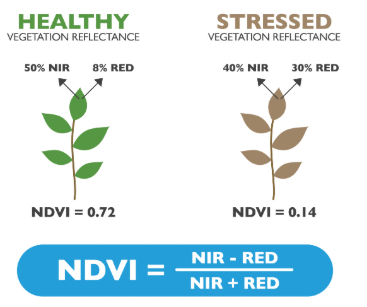
\includegraphics[width=0.6\textwidth]{image.png}
    \caption{Przykład interpretacji NDVI: Zielona, zdrowa roślina (NDVI = 0{,}72) ma wysoką wartość NIR i niską RED, natomiast roślina zestresowana (NDVI = 0{,}14) ma niższy NIR i wyższy RED.}
    \label{fig:ndvi_example}
\end{figure}
\noindent
-- wartość odbicia w bliskiej podczerwieni (np. pasmo B8 w SeŹródło: \cite{agricolus_ndvi_img}


\section{Zarys implementacji}
\label{sec:implementation}

System do analizy zmian wegetacji na podstawie zobrazowań Sentinel-2 zostanie zaprojektowany jako aplikacja modułowa, umożliwiająca łatwą rozbudowę i skalowanie. Poniżej przedstawiono główne założenia implementacyjne:

\subsection{Architektura systemu}
System będzie składał się z następujących głównych komponentów:
\begin{itemize}[leftmargin=*]
    \item \textbf{Moduł pobierania danych} -- automatyczne pobieranie i wstępne przetwarzanie zobrazowań Sentinel-2 z repozytoriów (np. Copernicus Open Access Hub).
    \item \textbf{Moduł przetwarzania równoległego} -- obliczanie wskaźników NDVI i NDMI na wielu rdzeniach CPU.
    \item \textbf{Moduł analizy i wizualizacji} -- generowanie map, wykresów oraz interaktywna prezentacja wyników użytkownikowi.
    \item \textbf{Interfejs użytkownika (GUI)} -- aplikacja desktopowa umożliwiająca wybór obszaru analizy, parametrów oraz przeglądanie wyników.
    \item \textbf{Moduł eksportu danych} -- umożliwiający zapis wyników w formatach rastrowych (GeoTIFF) i graficznych.
\end{itemize}

\subsection{Przepływ działania systemu}
\begin{enumerate}[leftmargin=*]
    \item Użytkownik wybiera obszar zainteresowania (AOI) oraz zakres czasowy analizy.
    \item System pobiera odpowiednie zobrazowania Sentinel-2 i wykonuje ich wstępne przetwarzanie.
    \item Moduł przetwarzania równoległego oblicza wskaźniki NDVI i NDMI dla wybranych scen.
    \item Wyniki są analizowane i prezentowane w formie map oraz wykresów w interfejsie graficznym.
    \item Użytkownik może eksportować wyniki do plików lub przeprowadzić dodatkową analizę.
\end{enumerate}

\noindent Całość rozwiązania zostanie zaimplementowana w języku Python z wykorzystaniem bibliotek do przetwarzania danych geoprzestrzennych (Rasterio, GDAL), obliczeń numerycznych (NumPy), przetwarzania równoległego (multiprocessing), wizualizacji (Matplotlib) oraz budowy GUI (PyQt6 lub Tkinter).

\section{Wybrane Technologie}
\label{sec:technologies}
Poniższa tabela przedstawia wybrane technologie wraz z ich głównym zastosowaniem w projekcie.

\begin{table}[H]
    \centering
    \caption{Wybrane technologie i ich zastosowanie.}
    \label{tab:technologies}
    \begin{tabular}{>{\raggedright\arraybackslash}p{0.4\textwidth} >{\raggedright\arraybackslash}p{0.5\textwidth}}
        \toprule
        \textbf{Technologia} & \textbf{Zastosowanie w Projekcie} \\
        \midrule
        Język Programowania: Python & Główny język implementacji logiki aplikacji, obliczeń i GUI. \\
        \addlinespace
        Przetwarzanie Równoległe: \texttt{multiprocessing} (Python) & Równoległe wykonywanie obliczeń indeksów NDVI/NDMI na wielu rdzeniach CPU. \\
        \addlinespace
        Przetwarzanie Danych Geoprzestrzennych: Rasterio (z GDAL) & Odczyt, zapis i podstawowe operacje na danych rastrowych Sentinel-2 (format GeoTIFF). \\
        \addlinespace
        Obliczenia Numeryczne: NumPy & Wydajne operacje na tablicach (pikselach obrazów) podczas obliczania indeksów. \\
        \addlinespace
        Interfejs Graficzny Użytkownika (GUI): PyQt6 (lub Tkinter) & Tworzenie interaktywnego interfejsu dla użytkownika (wczytywanie danych, wybór AOI, wizualizacja). \\
        \addlinespace
        Wizualizacja Danych: Matplotlib & Wyświetlanie przetworzonych map NDVI/NDMI w interfejsie graficznym. \\
        \addlinespace
        Format Danych Wyjściowych: GeoTIFF & Standardowy format zapisu przetworzonych map geoprzestrzennych. \\
        \bottomrule
    \end{tabular}
\end{table}

\section{Uruchamianie Programu}
\label{sec:run}
Aplikacja zostanie napisana w języku Python i będzie przeznaczona do uruchamiania jako aplikacja desktopowa. Poniżej przedstawione zostaną ogólne kroki do uruchomienia programu oraz informacje o planowanej kompatybilności systemowej.

\subsection{Wymagania Wstępne}
Do uruchomienia aplikacji potrzebne będą:
\begin{itemize}[leftmargin=*]
    \item Zainstalowany Python (zalecana wersja 3.8 lub nowsza).
    \item Zainstalowane biblioteki Python, które zostaną wymienione w sekcji \ref{sec:technologies} (np. PyQt6/Tkinter, Rasterio, NumPy, Matplotlib). Zalecane będzie użycie menedżera pakietów pip: \texttt{pip install -r requirements.txt} (plik \texttt{requirements.txt} zostanie dostarczony wraz z kodem źródłowym).
\end{itemize}

\subsection{Instrukcja Uruchomienia}
Planowane kroki uruchomienia aplikacji:
\begin{enumerate}[leftmargin=*]
    \item Pobranie kodu źródłowego aplikacji.
    \item Otwarcie terminala lub wiersza poleceń w głównym katalogu projektu.
    \item Upewnienie się, że wszystkie zależności są zainstalowane (zgodnie z Wymaganiami Wstępnymi).
    \item Uruchomienie głównego pliku aplikacji Pythona, np. \texttt{python main.py} (nazwa pliku może ulec zmianie).
\end{enumerate}

\subsection{Kompatybilność Systemowa}
Planuje się, że aplikacja będzie kompatybilna z następującymi systemami operacyjnymi:
\begin{itemize}[leftmargin=*]
    \item \textbf{Windows:} Tak (planowane testy na Windows 10/11).
    \item \textbf{macOS:} Tak (oczekuje się działania, ewentualne drobne dostosowania związane z bibliotekami GUI lub ścieżkami zostaną wprowadzone w razie potrzeby).
    \item \textbf{Linux:} Tak (oczekuje się działania na większości dystrybucji, np. Ubuntu, Fedora; podobnie jak w macOS, ewentualne drobne kwestie konfiguracyjne zostaną rozwiązane).
\end{itemize}
\noindent Należy uwzględnić, że działanie interfejsu graficznego oraz niektórych bibliotek (np. GDAL, będącego zależnością Rasterio) może nieznacznie różnić się między systemami operacyjnymi. W przypadku problemów, sprawdzona zostanie dokumentacja poszczególnych bibliotek dla danego systemu.

\printbibliography[heading=bibintoc]

\end{document}
